\documentclass[border=5,convert={density=600,outext=.png}]{standalone}

\usepackage{tikz-cd}
%\tikzexternalize[
%    prefix={tikz_external/},
%    only named,
%]


\begin{document}

%\begin{tikzpicture}
%\begin{tikzcd}[row sep=3cm,column sep=2cm,shorten >= 4pt,shorten <=4pt]
%F(x)
%  \arrow[bend left=40]{r}{F(f)}[name=UF,below]{}
%  \arrow[bend right=40]{r}[swap]{F(g)}[name=DF]{}
%  \arrow[bend left=30]{d}{A(x)}[name=D1,below]{}
%  \arrow[bend right=30]{d}[swap]{B(x)}[name=D2]{}
%& F(y) 
%  \arrow[bend left=30]{d}{A(y)}[name=D3,below]{}
%  \arrow[bend right=30]{d}[swap]{B(y)}[name=D4]{} \\
%G(x)
%  \arrow[bend left=40]{r}{G(f)}[name=UG,below]{}
%  \arrow[bend right=40]{r}[swap]{G(g)}[name=DG]{}
%& G(y) \\
%\arrow[Rightarrow,to path=(UF) -- (DF)]{}
%\arrow[Rightarrow,to path=(UG) -- (DG)]{}
%\arrow[Rightarrow,shorten <=10pt,to path=(D1|-D2) -- (D2)]{}
%\arrow[Rightarrow,shorten <=10pt,to path=(D3|-D4) -- (D4)]{}
%\end{tikzcd}
%\end{tikzpicture}

%\begin{tikzpicture}[>=Stealth,->,line width=.7pt]
%\matrix [matrix of math nodes,
%column sep={1.5cm,between origins},
%row sep={2.2cm,between origins},
%nodes={circle, draw, minimum size=1cm}]
%{
%& |(1)| 1 &   & |(2)| 2 & \\
%&  & |(3)| 3 &  \\
%& |(6)| 6 &   & |(5)| 5 & \\
%&  & |(4)| 4 &   \\};
%\draw (1)--(2);
%\draw (3)--(2);
%\draw[transform canvas={xshift=2pt,yshift=2pt},shorten <= -1pt] (3)--(1);
%\draw[transform canvas={xshift=-2pt,yshift=-2pt},shorten <= -1pt] (1)--(3);
%\draw (3) -- (5);
%\draw (5) -- (6);
%\draw[transform canvas={xshift=2pt,yshift=-2pt},shorten >= -1pt] (4) -- (5);
%\draw[transform canvas={xshift=-2pt,yshift=2pt},shorten >= -1pt] (5) -- (4);
%\draw[transform canvas={xshift=2pt,yshift=2pt},shorten <= -1pt] (4) -- (6);
%\draw[transform canvas={xshift=-2pt,yshift=-2pt},shorten <= -1pt] (6) -- (4);
%\end{tikzpicture}

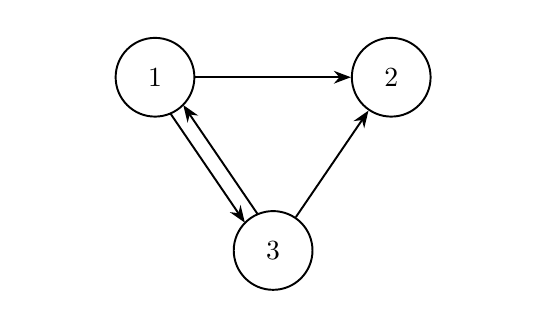
\begin{tikzpicture}[>=Stealth,->,line width=.7pt]
\matrix [matrix of math nodes,
column sep={1.5cm,between origins},
row sep={2.2cm,between origins},
nodes={circle, draw, minimum size=1cm}]
{
& |(1)| 1 &   & |(2)| 2 & \\
&  & |(3)| 3 &  \\};
\draw (1)--(2);
\draw (3)--(2);
\draw[transform canvas={xshift=2pt,yshift=2pt},shorten <= -1pt] (3)--(1);
\draw[transform canvas={xshift=-2pt,yshift=-2pt},shorten <= -1pt] (1)--(3);
\end{tikzpicture}

\end{document}
